\documentclass[eng,openany]{mgr}
\usepackage{listings}
\usepackage[english]{babel}
\usepackage{graphicx}
\usepackage{hyperref}
\usepackage{tabularx,colortbl} 
\usepackage{rotating}
\usepackage[utf8]{inputenc} 
\setlength\parindent{24pt}
\usepackage[parfill]{parskip}
\usepackage[table,kernelfbox,hyperref]{xcolor}
\usepackage{fancyhdr}
\usepackage{gauss}
%\usepackage[colorinlistoftodos]{todonotes}

\hypersetup{colorlinks=true}
\hypersetup{xurlbordercolor=red!70!black}
\hypersetup{xlinkbordercolor=blue!70!black}
\hypersetup{linkcolor=blue!60!black}
\hypersetup{urlcolor=red!50!black}
\hypersetup{citecolor=green!30!black}
\rfoot{Page \thepage}
\renewcommand\lstlistlistingname{List of Listings}
\newcommand{\linia}{\rule{\linewidth}{0.4mm}}

\definecolor{listlightgray}{gray}{0.93}

\newcommand{\lstsetmylst} {
\lstset{frame = tb,
breaklines=true,
framerule = 0.25pt,
float,
fontadjust,
backgroundcolor={\color{listlightgray}},
basicstyle = {\ttfamily\footnotesize},
identifierstyle = {\ttfamily},
stringstyle = {\ttfamily},
showstringspaces = false,
showtabs = false,
numbers = left,
numbersep = 6pt,
tabsize = 4,
language=C,
floatplacement=!h
}
}

\newcommand{\lstsetatc} {
\lstset{frame = tb,
breaklines=true,
framerule = 0.25pt,
float,
fontadjust,
backgroundcolor={\color{listlightgray}},
basicstyle = {\ttfamily\footnotesize},
keywordstyle = {\ttfamily\color{listkeyword}\textbf},
identifierstyle = {\ttfamily},
commentstyle = {\ttfamily\color{listcomment}\textit},
stringstyle = {\ttfamily},
showstringspaces = false,
showtabs = false,
numbers = left,
numbersep = 6pt,
numberstyle={\ttfamily\color{listnumbers}},
tabsize = 4,
language=C,
floatplacement=!h
}
}

\newcommand{\lstsetatbashnum} {
\lstset{frame = tb,
breaklines=true,
framerule = 0.25pt,
aboveskip=2ex,
float,
fontadjust,
backgroundcolor={\color{listlightgray}},
basicstyle = {\ttfamily\footnotesize},
keywordstyle = {\ttfamily\color{listkeyword}\textbf},
identifierstyle = {\ttfamily},
commentstyle = {\ttfamily\color{listcomment}\textit},
stringstyle = {\ttfamily},
showstringspaces = false,
showtabs = false,
numbers = left,
numbersep = 6pt,
numberstyle={\ttfamily\color{listnumbers}},
tabsize = 4,
language=bash,
floatplacement=!h
}
}
\lstsetmylst
\author{Jaroslaw M. Szumega}
\title{}
\engtitle{}
\supervisor{Rafal Zdunek, D.Sc, K-4/W4}
\field{Electronics}
\specialisation{Advanced Applied Electronics}
\date{15.05.2017}
\begin{document}
\selectlanguage{english}
\maketitle
\tableofcontents
\newpage

\chapter{Solution to the given problems}
\begin{figure}[h]
\centering
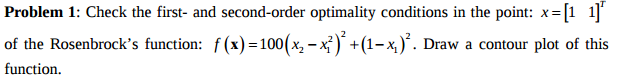
\includegraphics[width=0.7\linewidth]{screenshot001}
\label{fig:screenshot001}
\end{figure}

The first step will be expanding the given function, so further we can calculate the derivatives for gradient:\\
\begin{flalign*}
f(x) &= 100(x_2 - x_1^2)^2 + (1 - x_1)^2 \\
&= 100 (x_2^2 - 2x_2x_1^2 + x_1^4) + (1 - 2x_1 + x_1^2) \\
&= 100x_2^2 - 200x_2x_1^2 + 100x_1^4 + 1 - 2x_1 + x_1^2 \\
&= 100x_1^4 + x_1^2 - 2x_1 + 100x_2^2 - 200x_2x_1^2 + 1
\end{flalign*}
\\
\\
And the point to check is:\\
\begin{math}
x = [x_1\ x_2]^T = [1\ 1]^T
\end{math}

The First order optimality condition is:\\
\begin{flalign*}
\nabla f(x^*) &= 0\\ \\
\frac{\delta f(x)}{\delta x_2} &= 400x_1^3 + 2x_1 -2 - 400x_2x_1\\
&= 400 + 2 - 2 - 400 = 0\\ \\
\frac{\delta f(x)}{\delta x_1} &= 200x_2 - 200x_1^2\\
&= 200 - 200 =  0
\end{flalign*}

In given point x = [1 1] the first--order optimality condition is fulfilled.

The Second order optimality condition is:\\
\begin{flalign*}
\nabla f(x^*) &= 0\ (calculated\ in\ previous\ step)\\ \and
\nabla^2 f(x^*)\ &= positive\ semi-definite\ matrix\\ \\
\nabla^2 f(x^*)\ &= 
\begin{bmatrix}%
\frac{\delta^2 f(x)}{\delta x_1^2} & \frac{\delta^2 f(x)}{\delta x_1x_2}\\
\frac{\delta^2 f(x)}{\delta x_1x_2} & \frac{\delta^2 f(x)}{\delta x_2^2}
\end{bmatrix}\\
&=
\begin{bmatrix}%
1200x_1^2 + 2 - 400x_2& - 400x_1\\
-400x_1& 200
\end{bmatrix}\\
for\ point\ [1\ 1] &=
\begin{bmatrix}%
1200 + 2 - 400& - 400\\
-400& 200
\end{bmatrix}\\
H &=
\begin{bmatrix}%
802& -400\\
-400& 200
\end{bmatrix}
\end{flalign*}
As it can be noticed, all principal minors are positive ($H_{1,1}\ and\ H_{2,2}$). Therefore the $H(x_*)$ is positive semi-definite.\\
\\
Octave code below was written to plot contour for this task.
\begin{lstlisting}
pkg load symbolic

syms x1 x2
f = @(x1,x2) 100.*(x2 - x1.^2).^2 + (1 - x1).^2;

ezcontour(f,[-3,3])
\end{lstlisting}

\begin{figure}[h]
\centering
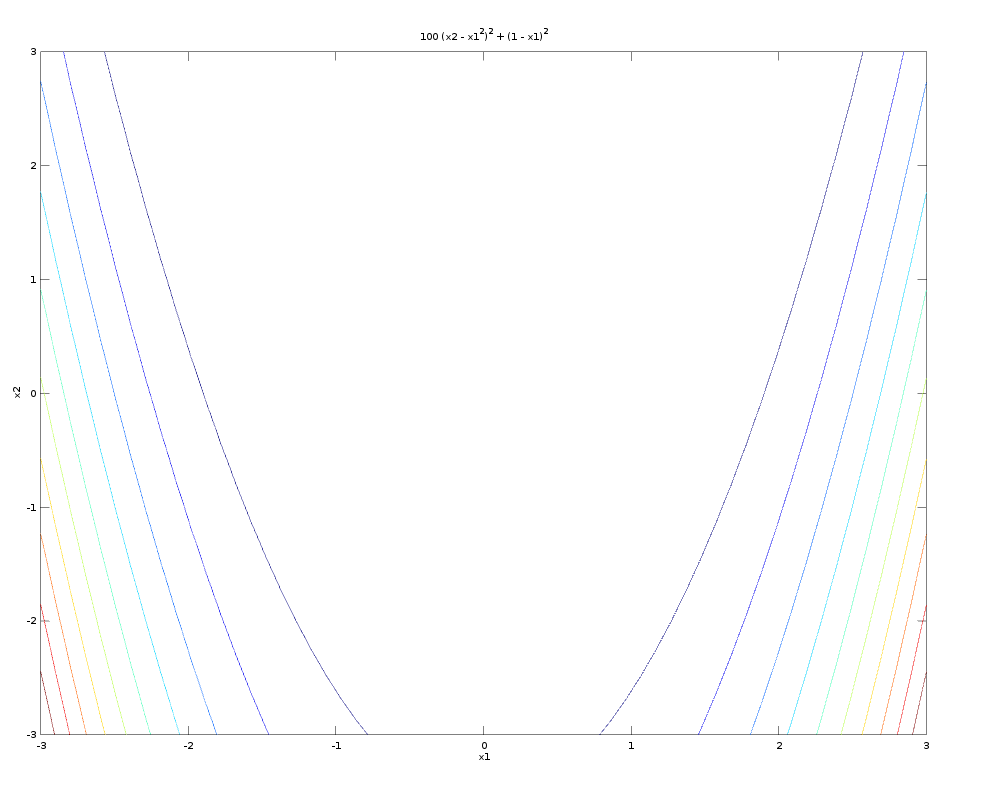
\includegraphics[width=0.7\linewidth]{screenshot002}
\caption{Contour plot of given function.}
\label{fig:screenshot002}
\end{figure}
\newpage
\begin{figure}[h]
	\centering
	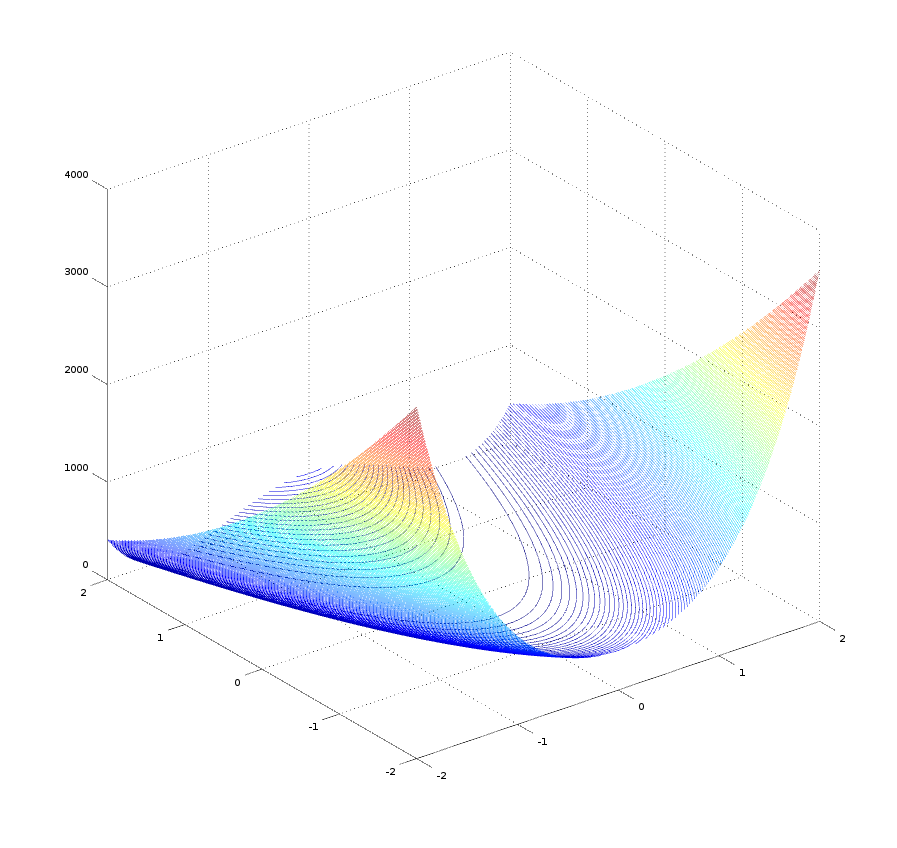
\includegraphics[width=0.7\linewidth]{screenshot007}
	\caption{Contour plot of function in 3D version.}
	\label{fig:screenshot007}
\end{figure}

\newpage

\begin{figure}[h]
	\centering
	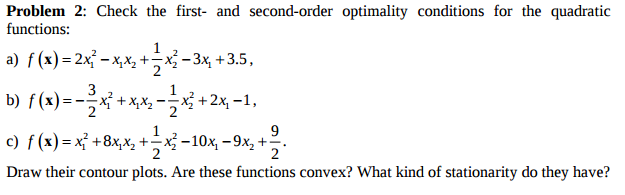
\includegraphics[width=0.7\linewidth]{screenshot003}
	\label{fig:screenshot003}
\end{figure}
Just like in the first task, we need to calculate the gradient and Hessian.//
Then it can be determined which type of stationarity the functions have.
\textbf{Point a)}
\\
\begin{align*}
f(x) &= 2 x_{1}^{2} - x_{1} x_{2} - 3 x_{1} + \frac{x_{2}^{2}}{2} + 3.5\\
\nabla f(x^*) &= 0\\ \\
\frac{\delta f(x)}{\delta x_2} &= 4 x_{1} - x_{2} - 3
\\
\frac{\delta f(x)}{\delta x_1} &= - x_{1} + x_{2}
\\
\end{align*}
To ensure the equality to zero, we can calculate that stationary point shall be:
\begin{align*}
x_1\ &=\ 1\\
x_2\ &=\ 1
\end{align*}

Now we will calculate the Hessian:
\begin{flalign*}
\nabla f(x^*) &= 0\ (calculated\ in\ previous\ step)\\ \and
\\
\nabla^2 f(x^*)\ &= 
\begin{bmatrix}%
\frac{\delta^2 f(x)}{\delta x_1^2} & \frac{\delta^2 f(x)}{\delta x_1x_2}\\
\frac{\delta^2 f(x)}{\delta x_1x_2} & \frac{\delta^2 f(x)}{\delta x_2^2}
\end{bmatrix}\\
&=
\begin{bmatrix}%
4& - 1\\
-1& 1
\end{bmatrix}\\
H &=
\begin{bmatrix}%
4& - 1\\
-1& 1
\end{bmatrix}\\
\end{flalign*}
To establish the type of stationarity we need to check Hessian determinant and the values of principal minors:
\begin{align*}
det(H)\ =\ 4\ +\ 1\ =\ 5\ >\ 0\\
H_{1,1}\ =\ 1\ >\ 0\\
H_{2,2}\ =\ 4\ >\ 0\\
\end{align*}

The Hessian is strictly positive definite, so we have the minimizer at calculated point.\\
\\

\begin{figure}[h]
	\centering
	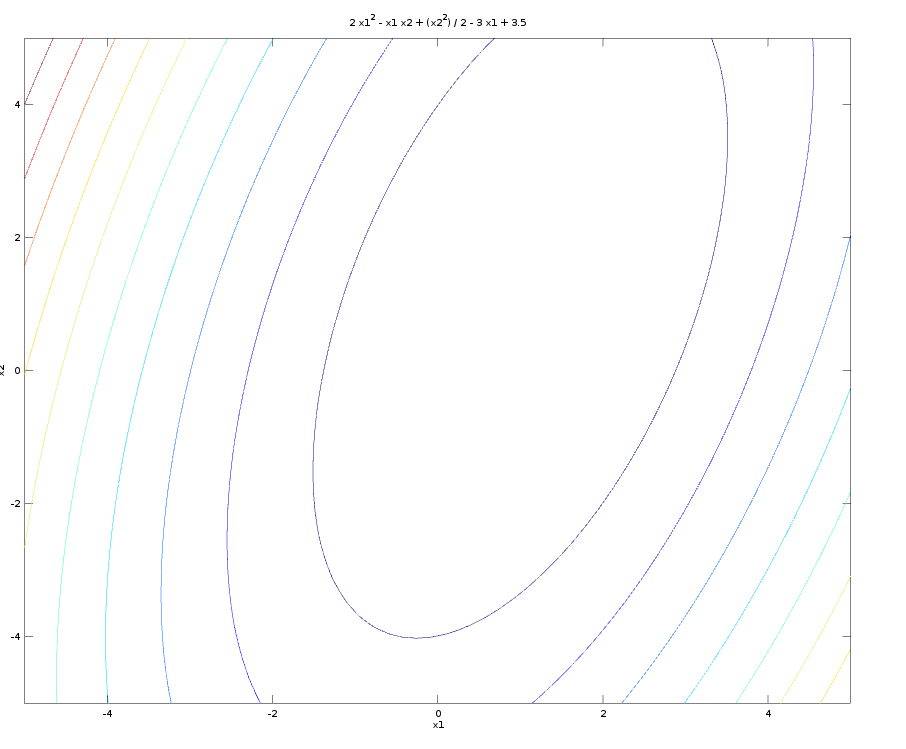
\includegraphics[width=0.7\linewidth]{screenshot004}
	\caption{Contour plot of point a) function.}
	\label{fig:screenshot004}
\end{figure}

\begin{figure}[h]
\centering
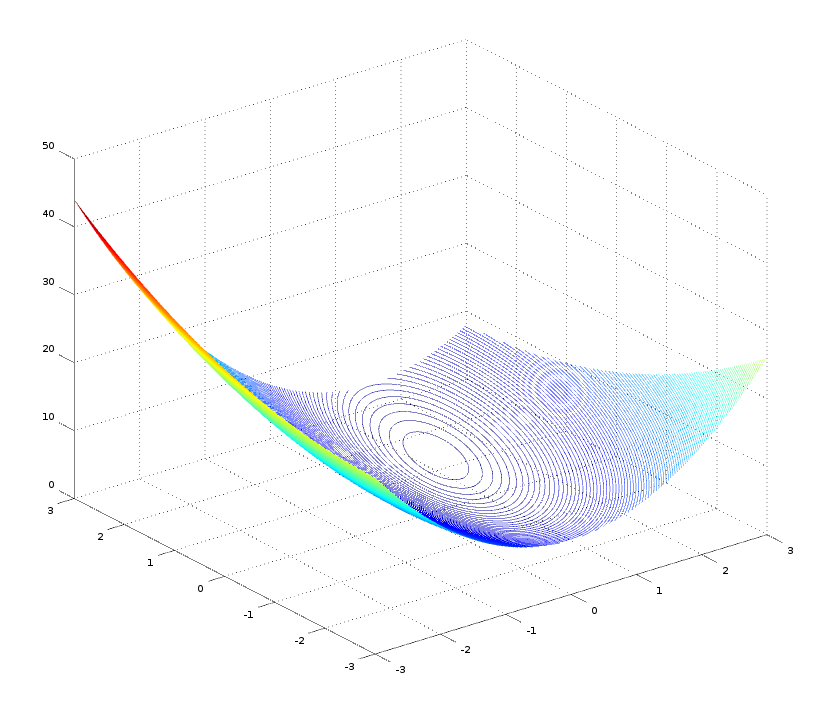
\includegraphics[width=0.7\linewidth]{screenshot008}
\caption{And its 3D version. We can notice the minimum.}
\label{fig:screenshot008}
\end{figure}

\clearpage

\textbf{Point b)}
\begin{align*}
f(x) &= - \frac{3 x_{1}^{2}}{2} + x_{1} x_{2} + 2 x_{1} - \frac{x_{2}^{2}}{2} - 1\\
\nabla f(x^*) &= 0\\ \\
\frac{\delta f(x)}{\delta x_2} &= - 3 x_{1} + x_{2} + 2
\\
\frac{\delta f(x)}{\delta x_1} &= x_{1} - x_{2}
\end{align*}
The calculated values for fulfilling the condition of $\nabla f(x^*) = 0$:
\begin{align*}
x_1\ &=\ 1\\
x_2\ &=\ 1
\end{align*}

Now we will calculate the Hessian:
\begin{flalign*}
\nabla f(x^*) &= 0\ (calculated\ in\ previous\ step)\\ \and
\\
\nabla^2 f(x^*)\ &= 
\begin{bmatrix}%
\frac{\delta^2 f(x)}{\delta x_1^2} & \frac{\delta^2 f(x)}{\delta x_1x_2}\\
\frac{\delta^2 f(x)}{\delta x_1x_2} & \frac{\delta^2 f(x)}{\delta x_2^2}
\end{bmatrix}\\
&=
\begin{bmatrix}%
-3& 1\\
1& -1
\end{bmatrix}\\
H &=
\begin{bmatrix}%
-3& 1\\
1& -1
\end{bmatrix}\\
\end{flalign*}
To establish the type of stationarity we need to check Hessian determinant and the values of principal minors:
\begin{align*}
det(H)\ =\ 3\ -\ 1\ =\ 2\ >\ 0\\
H_{1,1}\ =\ -1\ <\ 0\\
H_{2,2}\ =\ -3\ <\ 0\\
\end{align*}
The Hessian is strictly negative definite, The maximizer is present.
\\
\begin{figure}[h]
\centering
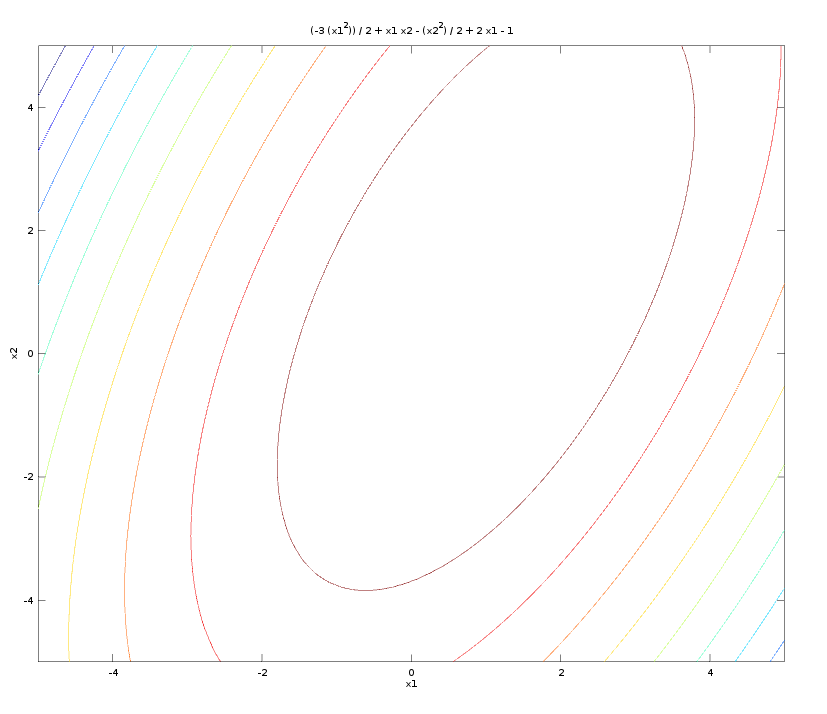
\includegraphics[width=0.7\linewidth]{screenshot005}
\caption{Contour plot of point b) function.}
\label{fig:screenshot005}
\end{figure}

\begin{figure}
\centering
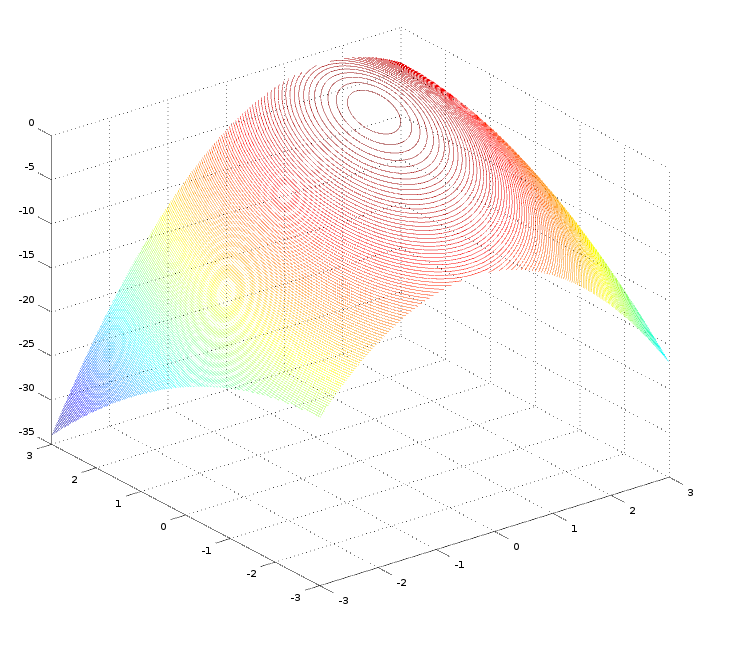
\includegraphics[width=0.7\linewidth]{screenshot009}
\caption{3D version with maximum observed.}
\label{fig:screenshot009}
\end{figure}


\clearpage
\textbf{Point c)}

In third point, the following function needs to be analyzed:
\begin{align*}
f(x) &= x_{1}^{2} + 8 x_{1} x_{2} - 10 x_{1} + \frac{x_{2}^{2}}{2} - 9 x_{2} + 4
\end{align*}

The task routine remains all the same as before:
\begin{align*}
\nabla f(x^*) &= 0\\ \\
\frac{\delta f(x)}{\delta x_2} &= 2 x_{1} + 8 x_{2} - 10
\\
\frac{\delta f(x)}{\delta x_1} &= 8 x_{1} + x_{2} - 9
\\
\end{align*}
To ensure the equality to zero, we can calculate that stationary point shall be:
\begin{align*}
x_1\ &=\ 1\\
x_2\ &=\ 1
\end{align*}

Now we will calculate the Hessian:
\begin{flalign*}
\nabla f(x^*) &= 0\ (calculated\ in\ previous\ step)\\ \and
\\
\nabla^2 f(x^*)\ &= 
\begin{bmatrix}%
\frac{\delta^2 f(x)}{\delta x_1^2} & \frac{\delta^2 f(x)}{\delta x_1x_2}\\
\frac{\delta^2 f(x)}{\delta x_1x_2} & \frac{\delta^2 f(x)}{\delta x_2^2}
\end{bmatrix}\\
&=
\begin{bmatrix}%
2& 8\\
8& 1
\end{bmatrix}\\
H &=
\begin{bmatrix}%
2& 8\\
8& 1
\end{bmatrix}\\
\end{flalign*}
To establish the type of stationarity we need to check Hessian determinant and the values of principal minors:
\begin{align*}
det(H)\ =\ 2\ -\ 64\ =\ -62\ <\ 0\\
\end{align*}
The determinant of Hessian is smaller than zero -- at this point we know that the critical point of function is a saddle point.
\\


\begin{figure}[h]
\centering
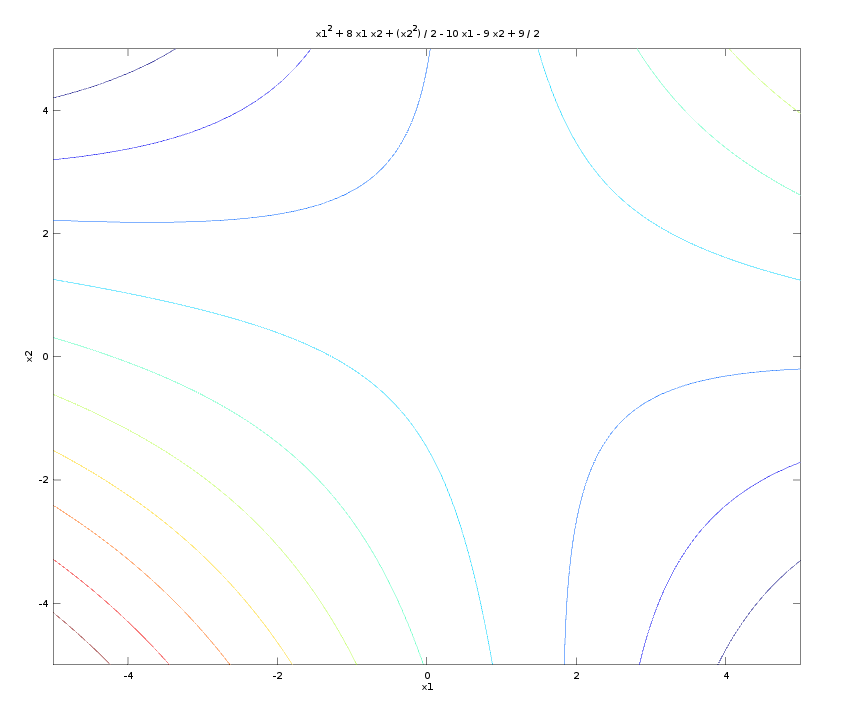
\includegraphics[width=0.7\linewidth]{screenshot006}
\caption{The contour plot of point c) function.}
\label{fig:screenshot006}
\end{figure}

\begin{figure}[h]
\centering
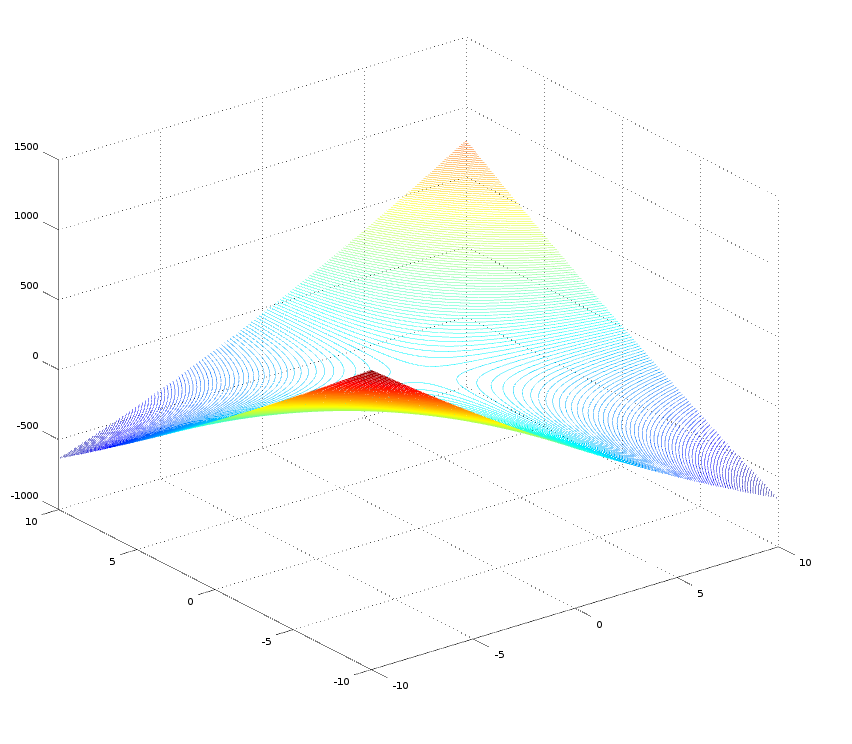
\includegraphics[width=0.7\linewidth]{screenshot010}
\caption{Visualization of point c) saddlepoint.}
\label{fig:screenshot010}
\end{figure}

\clearpage
\begin{figure}[h]
\centering

\includegraphics[width=0.7\linewidth]{screenshot011}
\label{fig:screenshot011}
\end{figure}

To ensure the function is convex, the presented matrix:\\
\begin{math}
\begin{bmatrix}
\alpha & 1 & 1\\
3& 2& 1\\
2& 2& 3\\
\end{bmatrix}
\end{math}
has to be strictly positive--definite.
Following this requirements, it needs to fulfill the following conditions:
\begin{itemize}
	\item matrix determinant > 0,
	\item first principal minor > 0.
\end{itemize}
So now we establish the determinant:\\
\begin{align*}
det(G) &= 6\alpha + 2 + 6 -4 - 2\alpha - 9\\
 &= 4 \alpha - 5
 \\
 4\alpha -5 &> 0\\
 \alpha &> 5/4
\end{align*}

And the first principal minor:\\
\begin{align*}
det(M1) &= 2\alpha - 3\\
\\
2\alpha -3 &> 0\\
\alpha &> 3/2
\end{align*}

In the end, if $alpha > 1.5$, then the given function will be convex.

\clearpage
\chapter{Listings of algorithms}
\section{Coded selected algorithms}
Algorithm 1 - Simplex algorithm\\ 
\begin{lstlisting}

\end{lstlisting}
\newpage
Algorithm 2 - Revised Simplex algorithm\\
\begin{lstlisting}

\end{lstlisting}
\begin{thebibliography}{8}
\addcontentsline{toc}{chapter}{Bibliography}
%\addcontentsline{toc}{section}{Literatura}
\bibitem{luenberger}
Luenberger, D. G., \& Ye, Y. (2015). Linear and nonlinear programming (Vol. 228). Springer.
\bibitem{zdunek}
Zdunek R., Optimization Methods - lecture slides.
\end{thebibliography}

\end{document}

